\chapter{Background}
\label{background}
\iffalse
\begin{itemize}
    \item Domain
    \begin{itemize}
        \item Network Security
        % Source: netsec: Network Secutity Basics: https://ieeexplore.ieee.org/abstract/document/1556540
        % Source: honeypot: Honeypot in network security: a survey: https://dl.acm.org/doi/abs/10.1145/1947940.1948065
        % Source: cryptography: Importance of Cryptography in Network Security: https://ieeexplore.ieee.org/abstract/document/6524439
        % Source: games: Bridging Game Theory and Cryptography: Recent Results and Future Directions: https://link.springer.com/chapter/10.1007/978-3-540-78524-8_15
        % Source: goals: An Ontology for Network Security Attacks: https://link.springer.com/chapter/10.1007/978-3-540-30176-9_41
        \item Edge-Computing
        % Source: edgecomputing: The promise of edge computing: https://ieeexplore.ieee.org/abstract/document/7469991
    \end{itemize}
    \item Enabling technologies
    \begin{itemize}
        \item SDN
        % Source: sdn: SDN survey: https://www.sciencedirect.com/science/article/abs/pii/S1084804516300297
        % Source: openflow: OpenFlow Switch Specification: https://opennetworking.org/wp-content/uploads/2014/10/openflow-switch-v1.5.1.pdf
        \item NFV
        % Source: nfv: NFV survey: https://www.sciencedirect.com/science/article/abs/pii/S1389128618300306
        \item SFC
        % Source: sfc: SFC survey: https://www.sciencedirect.com/science/article/abs/pii/S1084804516301989
        % Source: rfc7665: Service Function Chaining (SFC) Architecture: https://datatracker.ietf.org/doc/html/rfc7665
        \item VPN
        % Source: vpn: https://link.springer.com/article/10.1023/B:PNET.0000026887.35638.ce
        % Source: wireguard: https://www.wireguard.com/papers/wireguard.pdf
        % Source: openvpn: https://openvpn.net/images/pdf/OpenVPN_WhitepaperJuly2010.pdf
        \item MPLS
        % Source: rfc3031: RFC: https://datatracker.ietf.org/doc/html/rfc3031
        \item 2PCP
        % Source: 2pcp: https://dl.acm.org/doi/10.1145/850770.850772
    \end{itemize}
    \item Concepts
    \begin{itemize}
        \item QoS
        % Source: qos: A QoS architecture: https://dl.acm.org/doi/10.1145/185595.185648 (includes loss rate, throughput, jitter, delay within flows)
        % serv: IntServ and DiffServ: https://ieeexplore.ieee.org/abstract/document/891025
        % rfc791 (IP Protocol), rfc1633 (IntServ), rfc2474 (DiffServ)
        \item Network Slicing
        % Source: slicing: Overview of network slicing in the 5G context: https://ieeexplore.ieee.org/abstract/document/8685766
    \end{itemize}
\end{itemize}
\fi
Considering our remote surgery example and the threats we face, we now want to establish protections against these threats. To provide accurate protections we first have to analyze our domain. To do this, we will talk a bit about network security and edge computing in general. We will then focus on common concepts that can help us secure our communication, investigating quality of service (QoS) and network slicing. After this we will have a closer look on technologies that can help us along the way to realize the aforementioned concepts.
%In this chapter we will establish some common terms concerning the technical background of this thesis. First we will describe our domain of network security and edge computing, before introducing key technologies that have been used such as software defined networks (SDN), network function virtualization (NFV), service function chaining (SFC), virtual private networks (VPN) and multi protocol label switching (MPLS). Lastly we will focus on concepts like quality of service (QoS) and network slicing.

%\cgn{The current content of the background already contain good building blocks. However, it is hard to see the coherent connections between the blocks. I suggest a different order of writing: \begin{enumerate}
%    \item Use case: Human-Machine (or robot) interaction -- HCI (?) -- because networks are built for a purpose. And the purpose here is real-time communication between humans and robots, requiring multiple modalities (video, video, control, haptics, etc.). Multiple modalities with different requirements on bandwidths, delay, jitter, etc. raise the need for QoS and slicing.
%    \item Network domains and edge computing: to enable low-latency communication with direct edge-to-edge connections via autonomous systems. This sections, therefore, includes enabling technologies, such as NFV/SDN
%    \item MPLS (for tunneling / routing between AS) and VPN
%    \item Service differentiation (QoS, slicing)
%    \item (Network) Security, especially for mission critical use cases. At this point, it is natural to discuss the (security) requirements for the systems or networks you will discuss in Related work.
%\end{enumerate}
%By the way, I am unsure about the role of 2PCP and SFC in this thesis. However, it is possible that I didn't read it through. Therefore, as long as you can find a logical order for them, it should be good.
%}
%\cfw{I tried to spin the order by the three categories I used, structuring the content by the similarity of role in this thesis. Maybe the story reference could be placed in the beginning of the background and I could introduce the story as motivation in the introduction. I guess I could still spin the story in a way that it makes sense to begin with network security though, because consequences of failure could have been averted by designing the network with security in mind, introducing our domain. Then we can go to edge-computing to understand in which domain we are working. ("But to understand how we can secure our communications in the future, we must first understand or domain...") Then I could move up the concepts to say "this is how we could have had more security" and then state the building blocks (enabling technologies) that will help us build a better solution. This way I could connect all the blocks with a story by stating their relevance in the beginning and providing some links. Does that sound like a good idea? :) }

\section{Domain}
Considering our domain we locate ourselves in the network security context. We will thus first shed some light on this topic, because without knowing what security is we can not claim that something is secure. Afterwards we will focus on our general network architecture that we wish to secure communications on, which is edge computing.

\subsection{Network Security}
In order to secure communications in a network, we have to first define what network security is. According to \cite{netsec}, network security can be viewed as a subset of computer security, focusing on network-perimeter and computer system security. Some means to achieve this include, but are not limited to, computer intrusion detection, traffic analysis and network monitoring. Computer intrusion detection can be realised by installing intrusion detection software on systems that should be protected or by deploying honeypots \cite{honeypot}. Honeypots are systems that are supposed to be targeted by attackers in order to detect and distract them. By using honeypots one can learn what the attacker is going to try and ideally deploy protective measures before the attacker reaches a real system that needs to be protected. Traffic analysis on the other hand can be used to detect attacks based on traffic shapes that are unusual compared to normal operation. The same applies to network monitoring which instead focuses on events in the network.

Another view on network security can be from the cryptographical standpoint \cite{netsec}. Cryptography plays a key role in network security, because it can be used to achieve four of the major goals of security in network contexts: confidentiality, integrity, authentication and non-repudiation \cite{cryptography}. In this context often times security games are played to define what an attacker may know or not know at a certain point of a secure protocol, e.g. a key exchange, and what the attacker can possibly guess \cite{games}. The assumption generally is, that while some parties are honest and behaving according to protocol, some malicious actors will participate in the protocol. These malicious actors should (hopefully) never reach their goal concerning the protection goals from above.

So while the two views presented so far are of different nature, what combines them is the set of major protection goals on a network. Here are some of the most noteworthy \cite{goals}:
\paragraph{Confidentiality} Information that is only meant to be viewed by certain parties must not be disclosed to other parties.
\paragraph{Integrity} Information has to be protected against modification or forgery by malicious actors.
\paragraph{Availability} Information has to be available according to the service specifications.
\paragraph{Controlled access} Actors must not be able to perform actions on objects they are not permitted to.
\paragraph{Non-repudiation} Actors must not be able to claim that they did not take part in an action.

\cts{one could argue that authentication is less of a goal than a service, but controlled access would be a goal (note the Schaefer/Rossberg book, which picks the five of CIA + controlled access + non-rep ;)}
\cfw{I did some research on the book and adapted the protection goals accordingly, while swapping out the source :)}

\paragraph{} Apart from this there also exist other security services, such as \textit{authentication} (All actors must be identifiable by all entities at all times) and \textit{authorization} (All actors have to be assigned an access policy at all times), which are requirements to integrity, controlled access and non-repudiation.

\cfw{Are these descriptions accurate?}

\subsubsection{Resilience}
Furthermore, resilience of networks can be an important goal \cite{resilience}. According to Trivedi et al. \cite{resilience}, resilience of a network or computer system is the combination of trustworthiness and tolerance.

\paragraph{Trustworthiness} consists of:
\begin{itemize}
    \item Dependability (How reliable is the system?)
    \item Security (Which risks does a system have?)
    \item Performability (How capable is a system?)
\end{itemize}

\paragraph{Tolerance} consists of:
\begin{itemize}
    \item Survivability (How likely will a system survive when target of an attack?)
    \item Disruption tolerance (How well does the system handle service disruptions?)
    \item Traffic tolerance (How much traffic can the system handle?)
\end{itemize}

\paragraph{}When one of the six components of resilience is impeded, the major protection goals might be compromised. This is why resilience should play a key role when designing networks and services.

\paragraph{}So as one can see, network security is a relatively complex topic with many different approaches, view angles and goals. But while different approaches exist, it is of critical importance today to design networks with security in mind. Network outages can cause a lot of damage to property or infrastructure, prompting for security-aware solutions in the current world of digitalization. In our example of a surgery, the outcome could even be worse than just monetary damage.

\subsection{Edge Computing}
In our use case, we wish to communicate between two networks that are connected via multiple other networks. This means that opposed to the centralized approach of communicating from a remote client to a centralized server, we are communicating from one remote client to another remote client. This offloads computation from central servers to the edges of the networks.

Edge computing \cite{edgecomputing} refers to this relatively new approach, performing computations at the network edges, closer to the end user. As previously mentioned, the internet of today still follows a mostly centralized approach with servers clustered in data centers while users remain at the edges of the network.

This provides some challenges to the network though, because the traffic has to be transported over long distances. This has significant impact on latency, bandwidth at central hubs, security and privacy. By moving the computational resources (e.g. servers) closer to the user at the network edge, we can reply to requests from the user with less delay, with less transportation distance (and thus cost) and with more security and privacy in mind due to decentralization.

This also reduces the possible single points of failure because there is no central infrastructure anymore that could render a service unusable for all users. Edge computing has gained additional traction in recent developments due to the emergence of IoT in our everyday lifes. With a lot of data being collected by IoT devices, edge computing can be used to bundle all traffic generated by a users IoT devices closer to their origin, reducing the overall load of networks and thus their operational cost.

\section{Concepts}
\label{bg_concepts}
Next, we will focus on the central concepts that we can use to secure our communications in the edge computing context. For this, we need to know what a good and stable communications channel is compared to a bad one. Therefore we will introduce quality of service (QoS) and different metrics associated with it. Afterwards we are going to establish network slicing as a concept to help us guarantee meeting certain QoS parameters for our communications, which will help us eliminate our threats later.

\subsection{Quality of Service (QoS)}
% TODO: Maybe find a better base source for this chapter? --> It is hard to find a good source for such an old and basic term, thus the IP has been included for intial references of latency (delay), throughput and loss rate (high-reliability). The main qos source mentions the 4 terms below (as many other papers do).
For now, we just talked about securing our communications to always have an usable connection. But so far we have not talked about how a connection can be guaranteed to remain usable at all times. For this, the concept of quality of service (QoS) has been created.

Quality of service \cite{qos, rfc791} refers to assigning traffic to flows for which certain guarantees are to be uphold. These guarantees are usually measured in different metrics, of which the major four are outlined here:
\paragraph{Latency} The two-way delay for a packet travelling from flow start to finish and back.
\paragraph{Jitter} The mean deviation of latency from the mean latency (standard deviation).
\paragraph{Throughput} The number of bits transferable in one direction via the traffic flow in a certain time.
\paragraph{Loss rate} The number of lost packets divided by the total amount of packets. The loss rate is especially relevant in contexts where data needs to be transmitted again when lost, because the lost data will then need to be requested again and will be delivered delayed, thus at least doubling the latency.

\paragraph{}Securing these guarantees is an important task in network security, as violation of them could result in service level agreements (SLAs) being broken and violation of availability as one of our main goals.

To determine the flow for a certain packet, two main approaches exist \cite{serv}:
\paragraph{IntServ} Integrated Services \cite{rfc1633} negotiate flows beforehand with all participating network nodes. Packets are then assigned to flows based on pre-negotiated parameters. The advantage of this approach is that bandwidth and other assigned guarantees can be planned by the participating network providers in advance.
\paragraph{DiffServ} Differentiated Services \cite{rfc2474} on the other hand match quality of service on a per packet basis, normally by using the IPv4/IPv6 differentiated services (DS) header field. The advantage of this approach is that it provides flexibility to the sender of packets who can assign priorities per packet. The disadvantage is of course that network operators can not plan ahead accurately before packets arrive and providing guarantees will be challenging.

\subsection{Network Slicing}
Now that we know what we can guarantee to a communication flow, we still have to technically be able to realize these guarantees. This is where the concept of network slicing comes into play.

Network Slicing \cite{slicing} refers to partitioning part of the resources of a network to new virtual networks. Partitioned resources can include network resources, computational resources and storage resources. The result are multiple virtual networks that each have a slice of the resources of the underlying network available and guaranteed to them. In order to guarantee these resources to the owners of a slice, the slices need to be isolated from a resource perspective.

The latest developments in the field are part of the 5G standard, where applications can request slices of network resources to leverage uninterrupted communication afterwards. Apart from 5G also other applications leverage this approach already, for example by partitioning network links on nodes with multiple virtual machines.

\section{Enabling technologies}
In our concepts (section \ref{bg_concepts}) we stated that we want to isolate communication flows by performing network slicing. But in order to create network slices, we need technologies supporting us at this task. We will first focus on how we can orchestrate such a dynamic network, focusing on software defined networking (SDN), network function virtualization (NFV) and synchronization paradigms such as the two-phase commit protocol (2PCP). Afterwards we will discuss some means to provide private and resource isolated communications through multiple networks in the form of virtual private networks (VPN).

\subsection{Software Defined Networking (SDN)}
When building network topologies, software defined networking \cite{sdn} has emerged as one of the most valuable tools to build networks dynamically and with less cost.
While traditionally specialized hardware was deployed for every use case, SDN provides a number of abstractions to build arbitrary virtual topologies on top of real-world topologies.
To achieve this, software defined networking partitions the network into three major planes:
\cts{is the notion of 'higher' and 'lower' layers useful in the context of SDN (Giang?)? For me when it comes to networking higher layers are those closer to the application and lower layers those closer to the medium (iso/osi, tcp/ip models). Not sure..}
\cfw{Ah, most likely not. But I can simply omit "lowest" like I now did below :)}
\cgn{SDN usually uses plane instead of layer}
\cfw{I changed "layer" to "part of the infrastructure" below - hopefully now everything is correct :)}

\begin{figure}[h]
  \centering
  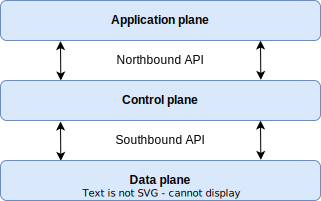
\includegraphics[width=\linewidth]{images/chapter_2/sdn.png}
  \caption[Software defined networking (SDN)]{The three planes of software defined networks: application plane, control plane and data plane. Application and control plane are connected via northbound APIs, while control and data plane are connected via southbound APIs like OpenFlow.}
  \label{fig:sdn}
\end{figure}

\paragraph{Data plane} This is the part of the infrastructure actually performing the work on the data to be transmitted. It is usually being realized by switches or other hardware that is used to perform work on the network traffic itself.

\paragraph{Control plane} The control plane consists of SDN controllers that instruct the data plane components on how to handle data via a so called southbound API. The data plane components will also contact the control plane when instructions for a certain type of traffic are needed that no rules have been defined for yet.

A commonly used protocol and the defacto standard for this southbound API is called OpenFlow \cite{openflow} and is currently supported by a wide range of SDN capable switches. With OpenFlow, traffic is being classified into flows via flow matching tables. After traffic has been assigned to a flow, the actions that have been defined for this flow will be applied on the traffic by the data plane components. Actions include dropping traffic, queuing traffic, outputting traffic on a specific port and modifying traffic in various ways.

\paragraph{Application plane} This plane is used to configure the SDN controllers via a northbound API. This can include end applications and users that want to manage and monitor the network.

\paragraph{}These three planes can also been seen in figure \ref{fig:sdn}.

\subsection{Network Function Virtualization (NFV)}
Closely related to SDN is the concept of network function virtualization \cite{nfv}. Network functions are components taking a specific role in a network, such as a switch which would forward or reshape traffic. Originally a lot of proprietary network functions were used to create larger networks. This resulted in a difficulty to manage the resulting networks. The proposed solution proposed for this is virtualization, so that individual network functions are decoupled from their hardware and executed in a virtual environment. The resulting network functions are called virtual network functions (VNFs) and can be orchestrated with ease to build complex topologies and integrations on a network level. Virtual network functions can thus be used as building blocks for software defined networks.

%\subsection{Service Function Chaining (SFC)}
%In order to interconnect our virtual network functions mentioned previously, service function chaining \cite{sfc} has emerged to connect different network functions to each other. According to Bhamare et al. \cite{sfc}, it is thus a key enabler for network function virtualization. The problem without service function chaining is, that network functions need to be linked to each other statically by providers. This provides significant effort to the network administrator to configure each connection manually in a static environment. With service function chaining, a virtualized software defined infrastructure is created connecting one network function to another, effectively forming a chain of service functions. To achieve the connections, a service function chaining architecture is used, of which multiple approaches and implementations currently exist. A common approach suggested by RFC 7665 \cite{rfc7665} is to encapsulate packets with an additional header (or additional information) that specifies the service function that the traffic should be steered towards. This header can either be added by a service function that is aware of the chain, or if the service function is not chain-aware it can be added after leaving the service function by the next network device the packet traverses to achieve easier routing of traffic. The standard also warns though (in section 5.6), that this could lead to a decrease in the maximum transmission unit (MTU), the maximum size the content of a packet may have on the network.

%\cts{two things: (1) are we using service function chaining later? I wouldn't introduce it otherwise.
%(2) mini English writing primer: text is structured in sentences, paragraphs, subsections, sections, and chapters. Each sentence should contain exactly one (and no more) statement. Each paragraph should group the statements that explain/discuss one (and no more) atomic concept/thought/idea. (Sub)sections group the paragraphs that discuss/explain one complex concept/thought. The abstraction layer throughout all paragraphs of one section should be identical (abstract vs technical vs detailed vs formal-with-variables/equations).
%The paragraph in 2.2.3 is too complex as it discusses different aspects of SFC. If we keep it, it should be cut to several paragraphs. ((2) is relevant for the entire thesis, of course ;-p)}

%\cfw{I will split the topic up, if we keep it. We currently use parallel structures to SFC in our thesis, so it is really only mentioned in one sentence in the design. All the VNFs from the application are usually adressed directly without SFC. But on the data layer, the MPLS tag with slice id and tunnel id can be viewed as service function chaning, as the slice id specifies which starting VPN gateway and which host the packet should be routed towards, while the tunnel id specifies which ending VPN gateway a packet should be routed towards. So in a sense we are building a service function chain with every slice, but maybe this can already be encompassed by the MPLS label paragraph and we can remove SFCs all together. I just wanted to mention them for reference, but am also not an expert on this topic. So in this sense, do you think it makes sense to keep it here or should I remove it all together?}

\subsection{Two-phase commit protocol (2PCP)}
Now that we know how we can orchestrate our network components by using software defined networking (SDN) and virtual network functions (NFVs), we can focus on synchronization between our networks. In our example of a remote surgery we need to have multiple networks working together in order to secure our communications. We will thus need to find a way to synchronize a network slice across all participating networks. For this, the two-phase commit protocol (2PCP) can be used.

The two-phase commit protocol \cite{2pcp} is a protocol used to synchronize state across transactions between multiple different participants.

The participant initiating a transaction is called the coordinator. The coordinator will send a change request to all participants of a transaction, which will take note of the changes and confirm whether their application is possible. This is also referred to as the voting phase.

Now the coordinator will proceed to the completion phase and can observe two different outcomes. The first possibility is that every participant responded that the change is possible. If so, the coordinator will send a commit message to all participants that will then apply the changes. This concludes the transaction. When the coordinator receives one failure or no reply from one of the participants though, the coordinator will abort the transaction and send rollback messages to all participants. All participants will then discard the changes, failing the transaction.

The two-phase commit protocol can not recover from a failure of the coordinator during the entire transaction or a participant during the commit phase, making it possible that an invalid state is left after a failure. We will talk about we how we can secure this later in the thesis.


\subsection{Virtual Private Networks (VPN)}
In order to isolate our communications and guarantee our network resources, we will use virtual private networks (VPNs).

A virtual private network \cite{vpn} is a virtual network overlayed on top of a real-world network providing private communication channels between their participants. With a lot of VPN approaches and implementations in existence, they can still be distinguished by classifying them per network layer. For example there are optical VPN on the physical network layer, tunnels like multi protocol label switching (MPLS, see section \ref{mpls}) on the ethernet layer and tunnels like wireguard \cite{wireguard} on the IP layer. While some only participate in routing (e.g. MPLS), others may also encrypt traffic (e.g. wireguard). Which VPN is the correct choice thus heavily depends on the use case.

\paragraph{Wireguard} One of the most prominent VPN solutions used today is wireguard \cite{wireguard}. Wireguard builds a tunnel between multiple participants (can be more than two) which then form a new virtual network. The participants can then communicate via the encrypted channels established by wireguard, which can thus traverse untrusted terrain without the fear of someone obtaining confidential information \cite{wireguard}.

Furthermore wireguard also provides protections against attacks on integrity of data according to their whitepaper \cite{wireguard}. An attacker may not produce ciphertext themselves, because traffic is encrypted and guessing valid ciphertext that will successfully decrypt "has a negligible probability" \cite{wireguardcrypto}. To achieve protection against replaying of packets, they use nonces that are never reused but accepted in a historical window of about 2000 entries \cite{wireguardproto}. When a packet has already been received, subsequent packets are thus dropped. An attacker may however drop certain packets if he chooses to do so, which the tunnel can of course not recover.

\paragraph{OpenVPN} Another commonly used implementation is OpenVPN \cite{openvpn}, which uses a slightly different approach. While OpenVPN also encrypts traffic, it can be used to connect to a remote network securely and reach nodes on this remote network. For this, OpenVPN uses a more traditional client server approach, where the server would expose devices on his network to the client, announcing routes to the client and forwarding traffic.

\paragraph{Multi Protocol Label Switching (MPLS)}
\label{mpls}
Multi protocol label switching \cite{rfc3031} was created to facilitate routing decisions within a network faster. Without MPLS each router in a network will form a routing decision based on a number of parameters from multiple packet headers by forming a longest match over addresses and comparing other header values before forwarding the packet. This deep inspection and matching of a packet can be omitted by labeling packets on the first hop. By assigning an MPLS label, encapsulating the original packet in an MPLS header, the following routers can perform their routing decision by simply investigating the label and forwarding the packet along the already well-known path. Stacking these labels is also supported, so one packet may be encapsulated multiple times. MPLS also creates the possibility to infer the class of traffic from a label by a router and thus perform decisions like precedence of a packet or discard thresholds. While this could also be performed by inspecting the packet headers closely in some cases, establishing a traffic class from a label is way less complex than a deep inspection of a packet, saving valuable computational time on core routers of a network.
